\documentclass{article}
\usepackage[utf8]{inputenc}
\usepackage{tikz}
\usetikzlibrary{shapes.geometric, arrows}

\tikzstyle{startstop} = [rectangle, rounded corners, text width = 3cm, minimum width=3cm, minimum height=1cm,text centered, draw=black, fill=red!30]

\tikzstyle{io} = [trapezium, trapezium left angle=70, trapezium right angle=110, minimum width=3cm, minimum height=1cm, text width = 3cm, text centered, draw=black, fill=blue!30]

\tikzstyle{process} = [rectangle, minimum width = 3cm,
minimum height = 1cm, text centered, text width = 3cm, draw = black, fill = orange!30]

\tikzstyle{decision} = [ellipse, minimum width = 3cm,
minimum height = 1cm, text centered, draw = black, fill =green!30]

\tikzstyle{arrow} = [thick, -> , >=stealth]

\begin{document}
\begin{centering}
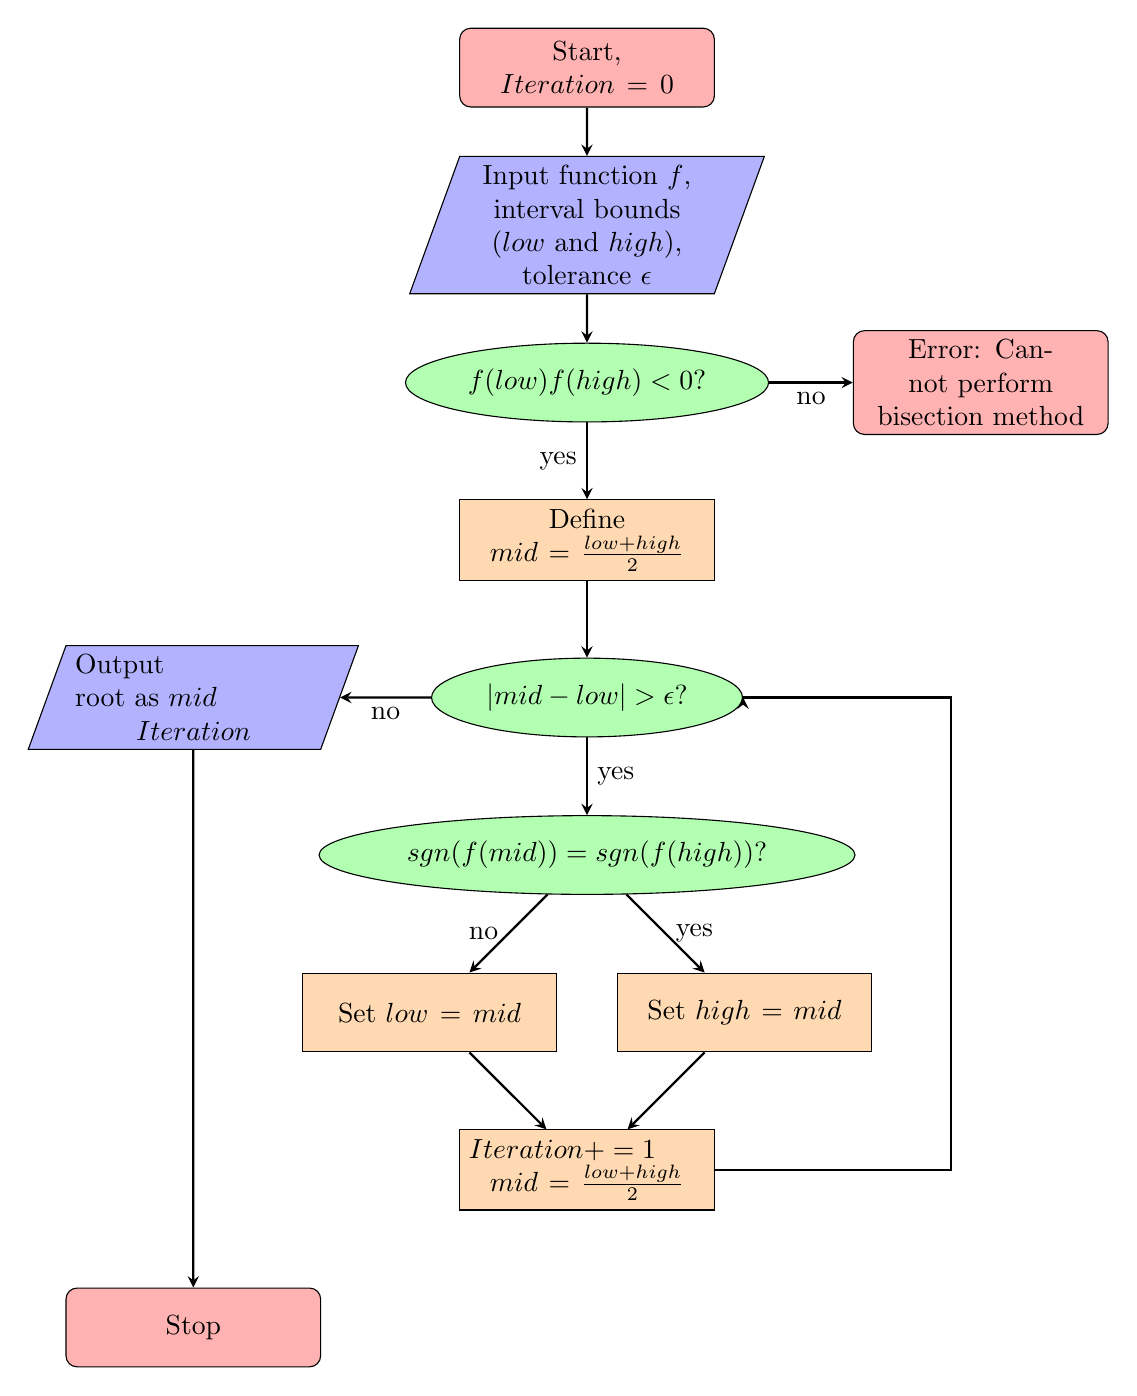
\begin{tikzpicture}[node distance = 2cm]

    
\node (start) [startstop] {Start, $Iteration = 0$};
\node (in1) [io, below of=start] {Input function $f$, interval bounds ($low$ and $high$), tolerance $\epsilon$};
\node (dec1) [decision, below of=in1] {$f(low)f(high)<0$?};

\node (err1) [startstop, right of = dec1, xshift = 3cm] {Error: Cannot perform bisection method};
\node (pro1) [process, below of=dec1] {Define $mid=\frac{low+high}{2}$};
\node (dec2) [decision, below of=pro1] {$|mid-low|>\epsilon$?};

\node (dec3) [decision, below of=dec2] {$sgn(f(mid))=sgn(f(high))$?};
\node (pro2a) [process, below of=dec3, xshift = 2cm] {Set $high=mid$};
\node (pro2b) [process, below of=dec3, xshift = -2cm] {Set $low=mid$};

\node (pro3) [process, below of = dec3, yshift = -2cm] {$Iteration+= 1\newline mid=\frac{low+high}{2}$};
%\node (pro2b) [process, right of=dec1, xshift = 2cm] {Process 2b text text text text text text text text};
\node (out1) [io, left of =dec2, xshift = -3cm] {Output $\newline$ root as $mid\newline$ $Iteration$};

\node (stop) [startstop, below of= out1, yshift = -6cm] {Stop};

\draw [arrow] (start) -- (in1);
\draw [arrow] (in1) -- (dec1);
\draw [arrow] (dec1) -- node[anchor = north]{no}(err1);
\draw [arrow] (dec1) -- node[anchor = east]{yes}(pro1);
\draw [arrow] (pro1) -- (dec2);
\draw [arrow] (dec2) -- node[anchor = north]{no}(out1);
\draw [arrow] (dec2) -- node[anchor = west]{yes}(dec3);

\draw [arrow] (dec3) -- node[anchor = east]{no}(pro2b);
\draw [arrow] (dec3) -- node[anchor = west]{yes}(pro2a);

\draw [arrow]  (pro2a) -- (pro3);
\draw [arrow]  (pro2b) -- (pro3);
%\draw [arrow]  (pro3.west) |- ([shift={(-5.5cm,0mm)}]pro3.west) |- ([shift={(-5cm,0mm)}]dec2.west) -| (dec2.west);
\draw [arrow]  (pro3.east) -- + (3,0) -- +(3,6) -| (dec2.east);
%\draw [arrow] (dec1.east) -- + (1,0) |- (pro3b)
\draw [arrow]  (out1) -- (stop);


\end{tikzpicture}

\end{centering}

\end{document}